% Options for packages loaded elsewhere
\PassOptionsToPackage{unicode}{hyperref}
\PassOptionsToPackage{hyphens}{url}
%
\documentclass[
  10,
]{article}
\usepackage{lmodern}
\usepackage{amsmath}
\usepackage{ifxetex,ifluatex}
\ifnum 0\ifxetex 1\fi\ifluatex 1\fi=0 % if pdftex
  \usepackage[T1]{fontenc}
  \usepackage[utf8]{inputenc}
  \usepackage{textcomp} % provide euro and other symbols
  \usepackage{amssymb}
\else % if luatex or xetex
  \usepackage{unicode-math}
  \defaultfontfeatures{Scale=MatchLowercase}
  \defaultfontfeatures[\rmfamily]{Ligatures=TeX,Scale=1}
\fi
% Use upquote if available, for straight quotes in verbatim environments
\IfFileExists{upquote.sty}{\usepackage{upquote}}{}
\IfFileExists{microtype.sty}{% use microtype if available
  \usepackage[]{microtype}
  \UseMicrotypeSet[protrusion]{basicmath} % disable protrusion for tt fonts
}{}
\makeatletter
\@ifundefined{KOMAClassName}{% if non-KOMA class
  \IfFileExists{parskip.sty}{%
    \usepackage{parskip}
  }{% else
    \setlength{\parindent}{0pt}
    \setlength{\parskip}{6pt plus 2pt minus 1pt}}
}{% if KOMA class
  \KOMAoptions{parskip=half}}
\makeatother
\usepackage{xcolor}
\IfFileExists{xurl.sty}{\usepackage{xurl}}{} % add URL line breaks if available
\IfFileExists{bookmark.sty}{\usepackage{bookmark}}{\usepackage{hyperref}}
\hypersetup{
  hidelinks,
  pdfcreator={LaTeX via pandoc}}
\urlstyle{same} % disable monospaced font for URLs
\usepackage[margin=1in]{geometry}
\usepackage{graphicx}
\makeatletter
\def\maxwidth{\ifdim\Gin@nat@width>\linewidth\linewidth\else\Gin@nat@width\fi}
\def\maxheight{\ifdim\Gin@nat@height>\textheight\textheight\else\Gin@nat@height\fi}
\makeatother
% Scale images if necessary, so that they will not overflow the page
% margins by default, and it is still possible to overwrite the defaults
% using explicit options in \includegraphics[width, height, ...]{}
\setkeys{Gin}{width=\maxwidth,height=\maxheight,keepaspectratio}
% Set default figure placement to htbp
\makeatletter
\def\fps@figure{htbp}
\makeatother
\setlength{\emergencystretch}{3em} % prevent overfull lines
\providecommand{\tightlist}{%
  \setlength{\itemsep}{0pt}\setlength{\parskip}{0pt}}
\setcounter{secnumdepth}{-\maxdimen} % remove section numbering
\usepackage{titlesec}
\usepackage{xcolor}
\usepackage[left=7.6cm,top=0.1cm,right=1cm,bottom=0.1cm,nohead,nofoot]{geometry}
\usepackage[document]{ragged2e}
\definecolor{title1}{HTML}{088A08}
\setmainfont{Montserrat}
\setsansfont{Arial}
\setmonofont{Arial}
\geometry{vmargin = 1cm, hmargin = 1cm}
\titleformat{\section}{\Large\fontsize{12}{14}\bfseries\sffamily\color{title1}}{}{0pt}{}
\ifluatex
  \usepackage{selnolig}  % disable illegal ligatures
\fi

\author{}
\date{\vspace{-2.5em}}

\begin{document}

\hypertarget{titulaciuxf3n-universitaria}{%
\section{TITULACIÓN UNIVERSITARIA}\label{titulaciuxf3n-universitaria}}

\hypertarget{bachiller-en-ing.-mecuxe1nica-de-fluidos-marzo---2020}{%
\subsection{Bachiller en Ing. Mecánica de Fluidos \textbar{} Marzo -
2020}\label{bachiller-en-ing.-mecuxe1nica-de-fluidos-marzo---2020}}

\hypertarget{formaciuxf3n-en-ing.-mecuxe1nica-de-fluidos-julio---2019}{%
\subsection{Formación en Ing. Mecánica de Fluidos \textbar{} Julio -
2019}\label{formaciuxf3n-en-ing.-mecuxe1nica-de-fluidos-julio---2019}}

\textbf{Universidad Nacional Mayor de San Marcos}\\
Formación en Recursos Hídricos, Hidrología e Hidráulica.

\hypertarget{formaciuxf3n-complementaria}{%
\section{FORMACIÓN COMPLEMENTARIA}\label{formaciuxf3n-complementaria}}

\begin{itemize}
\tightlist
\item
  Hidrología General: 40 h \textbar{} Agencia Nacional de Aguas (MOOC,
  Brasil)
\item
  Especialización en R: Básico, Intermedio y Avanzado: 84 h \textbar{}
  SDC
\item
  Modelos de Gestión de Recursos Hídricos en 5 Cuencas Hidrográficas del
  Perú: WEAP Y MODFLOW: 40 h \textbar{} TYPSA Perú.
\item
  Dipl. de Mod. Hidráulico e Hidrológico: 120 h \textbar{} CIDHMA.
\item
  Gestión de Proy. con Metodologías Agiles: 40 h \textbar{} Universitas
  Telefónica (MOOC, España)
\end{itemize}

\hypertarget{skills}{%
\section{SKILLS}\label{skills}}

\hypertarget{modelamiento}{%
\subsection{MODELAMIENTO}\label{modelamiento}}

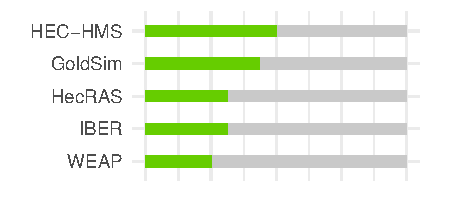
\includegraphics{resume_v01a_files/figure-latex/unnamed-chunk-1-1.pdf}

\hypertarget{cad-y-sig}{%
\subsection{CAD Y SIG}\label{cad-y-sig}}

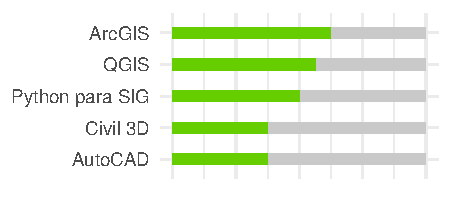
\includegraphics{resume_v01a_files/figure-latex/unnamed-chunk-2-1.pdf}

\hypertarget{estaduxedstica-y-leng.-de-programaciuxf3n}{%
\subsection{ESTADÍSTICA Y LENG. DE
PROGRAMACIÓN}\label{estaduxedstica-y-leng.-de-programaciuxf3n}}

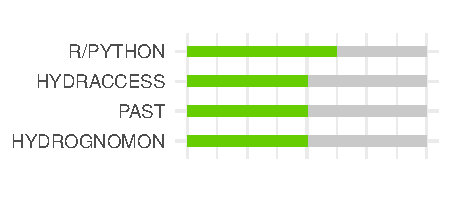
\includegraphics{resume_v01a_files/figure-latex/unnamed-chunk-3-1.pdf}

\newpage
\justify

\hypertarget{experiencia-profesional}{%
\section{EXPERIENCIA PROFESIONAL}\label{experiencia-profesional}}

\hypertarget{especialista-jr.-en-recursos-huxeddricos-uxe1rea-de-ciencias-del-agua}{%
\subsubsection{ESPECIALISTA JR. EN RECURSOS HÍDRICOS, ÁREA DE CIENCIAS
DEL
AGUA}\label{especialista-jr.-en-recursos-huxeddricos-uxe1rea-de-ciencias-del-agua}}

\textcolor{darkgray}{\textbf{SNC-LAVALIN, Perú}}

Recopilación, pre-proceso, proceso y análisis de datos hidroclimáticos
para caracterización climática, modelamiento hidrológico y análisis de
máximas avenidas, análisis de sequías, planes de gestión hídrica, uso de
lenguajes de programación (R y Python) para automatizar actividades, y
análisis de datos espaciales y no espaciales.

\hypertarget{ingeniero-jr.-en-recursos-huxeddricos-uxe1rea-de-geoingenieruxeda}{%
\subsubsection{INGENIERO JR. EN RECURSOS HÍDRICOS, ÁREA DE
GEOINGENIERÍA}\label{ingeniero-jr.-en-recursos-huxeddricos-uxe1rea-de-geoingenieruxeda}}

\textcolor{darkgray}{\textbf{SRK Consulting, Perú}}

Recopilación, pre-proceso, proceso y análisis de datos hidroclimáticos
para caracterización climática, modelamiento hidrológico y análisis de
máximas avenidas, análisis de sequías, planes de gestión hídrica, uso de
herramientas SIG para el análisis geoespacial y desarrollo de mapas
temáticos, modelamiento de balance de aguas en GoldSim, uso de lenguajes
de programación (R y Python) para automatizar actividades, y análisis de
datos espaciales y no espaciales.

\hypertarget{asistente-de-ingenieruxeda-dpto-de-ingenieruxeda-del-agua}{%
\subsubsection{ASISTENTE DE INGENIERÍA, DPTO DE INGENIERÍA DEL
AGUA}\label{asistente-de-ingenieruxeda-dpto-de-ingenieruxeda-del-agua}}

\textcolor{darkgray}{\textbf{TYPSA, Perú}}

Pre-proceso, proceso y análisis de datos hidroclimáticos para
modelamiento hidrológico, eventos extremos, planes de gestión hídrica,
Dibujante CAD de planos hidráulicos, abastecimiento y drenaje, SIG para
el análisis, proceso geoespacial en hidráulica e hidrología y creación
de mapas.

\hypertarget{asistente-en-recursos-huxeddricos}{%
\subsubsection{ASISTENTE EN RECURSOS
HÍDRICOS}\label{asistente-en-recursos-huxeddricos}}

\textcolor{darkgray}{\textbf{TYPSA, Perú}}

Pre-proceso de datos hidroclimáticos para modelamiento: hidrológico,
eventos extremos y recursos hídricos, redacción y revisión parcial de
informes y anexos, procesamiento geoespacial usando herramientas SIG

\hypertarget{voluntario}{%
\subsubsection{VOLUNTARIO}\label{voluntario}}

\textcolor{darkgray}{\textbf{CIDIMF-UNMSM, Perú}}

Desarrollé programas para Hidrología Estadística usando R, Python y
MATLAB, Participé en la planeación y desarrollo de un sistema de riego
automatizado, brinde capacitación en Hidrología y afines.

\hypertarget{principales-proyectos}{%
\section{PRINCIPALES PROYECTOS}\label{principales-proyectos}}

\hypertarget{campauxf1a-de-aforo-muestreo-de-sedimentos-y-agua-ecuador}{%
\subsubsection{CAMPAÑA DE AFORO, MUESTREO DE SEDIMENTOS Y AGUA
\textbar{}
ECUADOR}\label{campauxf1a-de-aforo-muestreo-de-sedimentos-y-agua-ecuador}}

\textcolor{darkgray}{\textbf{\emph{U.M. Ruta de Cobre}}}

Soporte en el aforo de ríos y quebradas, toma de muestras de sedimentos
y agua en múltiples puntos de la microcuenca Chaucha (Ecuador).

\hypertarget{paquete-ideamr-colombia}{%
\subsubsection{Paquete IdeamR \textbar{}
COLOMBIA}\label{paquete-ideamr-colombia}}

\textcolor{darkgray}{\textbf{\emph{Software para la automatización de procesos hidrológicos}}}

ideamR es un paquete desarrollado en R para el manejo de datos
hidrometeorológicos de DHIME (IDEAM, Colombia). DHIME es un Sistema de
Información para el manejo de datos hidrológicos y meteorológicos de
Colombia. Enlace: \url{https://github.com/GeomarPerales/ideamR}

\newpage

\hypertarget{rpisco-peruxfa}{%
\subsubsection{RPisco \textbar{} PERÚ}\label{rpisco-peruxfa}}

\textcolor{darkgray}{\textbf{\emph{Software para la automatización de procesos hidrológicos}}}

RPisco es un paquete desarrollado en R con herramientas para extraer y
manipular datos climáticos de PISCO (SENAMHI, Perú). Enlace:
\href{https://github.com/GeomarPerales/RPisco}{RPisco}.

\hypertarget{estudio-hidroluxf3gico-y-anuxe1lisis-de-muxe1ximas-avenidas-colombia}{%
\subsubsection{ESTUDIO HIDROLÓGICO Y ANÁLISIS DE MÁXIMAS AVENIDAS
\textbar{}
COLOMBIA}\label{estudio-hidroluxf3gico-y-anuxe1lisis-de-muxe1ximas-avenidas-colombia}}

\textcolor{darkgray}{\textbf{\emph{U.M. Quinchia y La Perla}}}

Recopilación, pre-proceso, proceso y análisis de datos hidroclimáticos
para la caracterización hidroclimática, y análisis de máximas avenidas.

\hypertarget{recopilaciuxf3n-y-pre-proceso-de-informaciuxf3n-climuxe1tica-uzbekistuxe1n}{%
\subsubsection{RECOPILACIÓN Y PRE-PROCESO DE INFORMACIÓN CLIMÁTICA
\textbar{}
UZBEKISTÁN}\label{recopilaciuxf3n-y-pre-proceso-de-informaciuxf3n-climuxe1tica-uzbekistuxe1n}}

\textcolor{darkgray}{\textbf{\emph{Energía Solar}}}

Búsqueda, recopilación y proceso de información hidroclimática en bases
de datos extranjeras (en inglés). Revisión y análisis de la bibliografía
(Papers, informes y otros, en inglés).

\hypertarget{pre-proceso-y-anuxe1lisis-de-precipitaciuxf3n-maxima-peruxfa}{%
\subsubsection{PRE-PROCESO Y ANÁLISIS DE PRECIPITACIÓN MAXIMA \textbar{}
PERÚ}\label{pre-proceso-y-anuxe1lisis-de-precipitaciuxf3n-maxima-peruxfa}}

\textcolor{darkgray}{\textbf{\emph{Construcción del reemplazo del Pte. San Francisco en Ayacucho}}}

Responsable del pre-proceso, proceso y análisis de precipitación máxima
de 24 horas de diversas fuentes de información para el estudio de
máximas avenidas.

\hypertarget{entrega-del-4-informe-e-informe-final-de-recursos-huxeddricos-peruxfa}{%
\subsubsection{ENTREGA DEL 4° INFORME E INFORME FINAL DE RECURSOS
HÍDRICOS \textbar{}
PERÚ}\label{entrega-del-4-informe-e-informe-final-de-recursos-huxeddricos-peruxfa}}

\textcolor{darkgray}{\textbf{\emph{Gestión de Recursos Hídricos de 5 Cuencas Hidrográficas}}}

Responsable de la redacción parcial, revisión y entrega del Informe de
la Cuenca Nanay, planeamiento, gestión, preparación y entrega del
Informe más anexos respectivos.

\hypertarget{modelaciuxf3n-hidroluxf3gica-peruxfa}{%
\subsubsection{MODELACIÓN HIDROLÓGICA \textbar{}
PERÚ}\label{modelaciuxf3n-hidroluxf3gica-peruxfa}}

\textcolor{darkgray}{\textbf{\emph{Plan Maestro de drenaje pluvial de Piura}}}

Soporte en Modelación Hidrológica, geoprocesamiento de información
pluviométrica, modelación de caudales, delimitación de cuencas urbanas,
dibujante SIG.

\hypertarget{pre-proceso-y-anuxe1lisis-de-precipitaciuxf3n-maxima-g-peruxfa}{%
\subsubsection{PRE-PROCESO Y ANÁLISIS DE PRECIPITACIÓN MAXIMA \textbar{}
G \textbar{}
PERÚ}\label{pre-proceso-y-anuxe1lisis-de-precipitaciuxf3n-maxima-g-peruxfa}}

\textcolor{darkgray}{\textbf{\emph{Gestión de Recursos Hídricos de 5 Cuencas Hidrográficas}}}

Responsable del Pre-proceso y proceso de precipitación máxima de 24
horas para el estudio de máximas avenidas del Proyecto.

\hypertarget{proceso-de-informaciuxf3n-de-demandas-huxeddricas-g-peruxfa}{%
\subsubsection{PROCESO DE INFORMACIÓN DE DEMANDAS HÍDRICAS \textbar{} G
\textbar{}
PERÚ}\label{proceso-de-informaciuxf3n-de-demandas-huxeddricas-g-peruxfa}}

\textcolor{darkgray}{\textbf{\emph{Gestión de Recursos Hídricos de 5 Cuencas Hidrográficas}}}

Responsable de la coordinación, gestión y organización de equipos para
el pre-proceso de demandas hídricas, proceso y generación de bases de
datos de demandas hídricas.

\hypertarget{pre-proceso-de-informaciuxf3n-hidroclimuxe1tica-g-peruxfa}{%
\subsubsection{PRE-PROCESO DE INFORMACIÓN HIDROCLIMÁTICA \textbar{} G
\textbar{}
PERÚ}\label{pre-proceso-de-informaciuxf3n-hidroclimuxe1tica-g-peruxfa}}

\textcolor{darkgray}{\textbf{\emph{Gestión de Recursos Hídricos de 5 Cuencas Hidrográficas}}}

Responsable del Pre-proceso, generación y estructuración de bases de
datos hidroclimáticos para el modelamiento hidrológico y de recursos
hídricos de las cuencas del estudio.

\newpage

\hypertarget{actividades-de-divulgaciuxf3n}{%
\section{ACTIVIDADES DE
DIVULGACIÓN}\label{actividades-de-divulgaciuxf3n}}

\hypertarget{expositor}{%
\subsubsection{EXPOSITOR}\label{expositor}}

\textcolor{darkgray}{\textbf{Empresa HelpGIS, Perú}}

Webinar ``R y Python aplicados a la Hidrología'', 19-06-21.

\textcolor{darkgray}{\textbf{Empresa Hidroclic, Perú}}

Webinar ``Rompiendo Mitos en R aplicado a Hidrología'', 05-10-20.

Webinar ``R aplicado a Hidrología'', 29-09-20

\hypertarget{asociaciones-tuxe9cnicas}{%
\section{ASOCIACIONES TÉCNICAS}\label{asociaciones-tuxe9cnicas}}

\textcolor{darkgray}{\textbf{CIDIMF-UNMSM, Perú}}

\hypertarget{presidente}{%
\subsubsection{PRESIDENTE}\label{presidente}}

Dirección y gestión de diversas actividades de: divulgación,
capacitación y orientación en temas de Recursos Hídricos a los miembros
del Grupo Estudiantil CIDIMF y externos

\hypertarget{voluntario-1}{%
\subsubsection{VOLUNTARIO}\label{voluntario-1}}

Colabore en la gestión, organización y divulgación de eventos orientados
a los Recursos Hídricos, desarrollé habilidades de liderazgo y participe
en multiples actividades de divulgación.

\end{document}
